\begin{problem}
  {Q3(a)}
  ~\\
  \begin{center}
    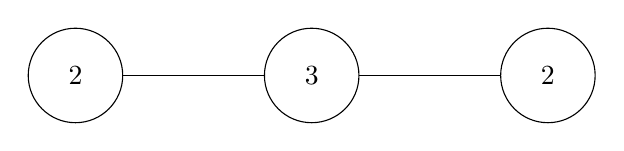
\begin{tikzpicture}[scale=0.2]
      \tikzstyle{every node}+=[inner sep=0pt]
      \draw [black] (5,0) circle (3);
      \draw (5,0) node {$2$};
      \draw [black] (20,0) circle (3);
      \draw (20,0) node {$3$};
      \draw [black] (35,0) circle (3);
      \draw [black] (35,0) node {$2$};
      \draw [black] (23,0) -- (32,0);
      \draw [black] (8,0) -- (17,0);
    \end{tikzpicture}
  \end{center}
  In this example, the middle node will be chosen and the two side nodes discarded for a total weight of $3$. \\
  If the middle node was discarded and the two side nodes chosen, the total weight would have been $4 > 3$. \\
\end{problem}
